\documentclass[journal]{IEEEtran}
\hyphenation{op-tical net-works semi-conduc-tor}
\usepackage{graphicx}
\graphicspath{{./images/}}

\begin{document}
\title{3D Indoor Mapping Using ROS and Microsoft Kinect Sensor}
\author{Chirag~Shah
        and~Srijal~Poojari}% <-this % stops a space
%\thanks{M. Shell was with the Department
%of Electrical and Computer Engineering, Georgia Institute of Technology, Atlanta,
%GA, 30332 USA e-mail: (see http://www.michaelshell.org/contact.html).}% <-this % stops a space
%\thanks{J. Doe and J. Doe are with Anonymous University.}% <-this % stops a space
%\thanks{Manuscript received April 19, 2005; revised August 26, 2015.}}

% note the % following the last \IEEEmembership and also \thanks - 
% these prevent an unwanted space from occurring between the last author name
% and the end of the author line. i.e., if you had this:
% 
% \author{....lastname \thanks{...} \thanks{...} }
%                     ^------------^------------^----Do not want these spaces!
%
% a space would be appended to the last name and could cause every name on that
% line to be shifted left slightly. This is one of those "LaTeX things". For
% instance, "\textbf{A} \textbf{B}" will typeset as "A B" not "AB". To get
% "AB" then you have to do: "\textbf{A}\textbf{B}"
% \thanks is no different in this regard, so shield the last } of each \thanks
% that ends a line with a % and do not let a space in before the next \thanks.
% Spaces after \IEEEmembership other than the last one are OK (and needed) as
% you are supposed to have spaces between the names. For what it is worth,
% this is a minor point as most people would not even notice if the said evil
% space somehow managed to creep in.


% The paper headers
\markboth{Journal of \LaTeX\ Class Files,~Vol.~14, No.~8, August~2015}%
{Shell \MakeLowercase{\textit{et al.}}: Bare Demo of IEEEtran.cls for IEEE Journals}
% The only time the second header will appear is for the odd numbered pages
% after the title page when using the twoside option.
% 
% *** Note that you probably will NOT want to include the author's ***
% *** name in the headers of peer review papers.                   ***
% You can use \ifCLASSOPTIONpeerreview for conditional compilation here if
% you desire.




% If you want to put a publisher's ID mark on the page you can do it like
% this:
%\IEEEpubid{0000--0000/00\$00.00~\copyright~2015 IEEE}
% Remember, if you use this you must call \IEEEpubidadjcol in the second
% column for its text to clear the IEEEpubid mark.



% use for special paper notices
%\IEEEspecialpapernotice{(Invited Paper)}




% make the title area
\maketitle

% As a general rule, do not put math, special symbols or citations
% in the abstract or keywords.
\begin{abstract}
This project deals with the exploring the ROS framework for development of a robotic system with various
sensors and actuators in order to understand the underlying concepts and to create a robot/quadcoptor
capable of forming a 3D map of a given environment using a depth camera (Microsoft Kinect).
\end{abstract}

% Note that keywords are not normally used for peerreview papers.
\begin{IEEEkeywords}
ROS, Robot Operating System, 3D-Mapping, Microsoft Kinect Sensor
\end{IEEEkeywords}


% For peer review papers, you can put extra information on the cover
% page as needed:
% \ifCLASSOPTIONpeerreview
% \begin{center} \bfseries EDICS Category: 3-BBND \end{center}
% \fi
%
% For peerreview papers, this IEEEtran command inserts a page break and
% creates the second title. It will be ignored for other modes.
\IEEEpeerreviewmaketitle


\section{Introduction}
\IEEEPARstart{A}{utonomous} robots operating in real life settings must be able to navigate in large, unstructured, dynamic and unknown spaces. To do so, they must build a map of their operating environment in order to localize itself in it, a problem known as Simultaneous localization and mapping (SLAM). 
\\

\hfill mds
 
\hfill October 30, 2017

%\section{Related Work}

\section{Major Components of Our System}

\subsection{Robot Operating System}
The Robot Operating System (ROS) is a framework for writing robot software. It is a set of utilities and libraries for implementing different kinds of functionality on robots. It is a collection of tools, libraries, and conventions that aim to simplify the task of creating complex and robust robot behavior across a wide variety of robotic platforms. It is not a programming language. 

A ROS system is comprised of a number of independent nodes, each of which communicates with the other nodes using a publish/subscribe messaging model. For example, a particular sensor’s driver might be implemented as a node, which publishes sensor data in a stream of messages. These messages could be consumed by any number of other nodes.
Note that nodes in ROS do not have to be on the same system or even systems of the same architecture. This makes ROS really flexible and adaptable to the needs of the user. ROS is open source, maintained by many people.
ROS starts with the ROS Master. The Master allows all other nodes to find and talk to each other. 

\subsubsection{roscore}
roscore is a service that provides connection information to nodes so that they can
transmit messages to one another. Every node connects to roscore at startup to register
details of the message streams it publishes and the streams to which it wishes to subscribe.
When a new node appears, roscore provides it with the information that it needs to form a
direct peer-to-peer connection with other nodes publishing and subscribing to the same
message topics. Every ROS system needs a running roscore, since without it, nodes
cannot find other nodes.
With knowledge of the location of roscore on the network, nodes register themselves at
startup with roscore and then query roscore to find other nodes and data streams by
name. Each ROS node tells roscore which messages it provides and which it would like
to subscribe to. roscore then provides the addresses of the relevant message producers
and consumers.

\subsubsection{Nodes}
A node is a process that performs computation. Nodes are combined together into a graph and communicate with one another using streaming topics, RPC services, and the Parameter Server. These nodes are meant to operate at a fine-grained scale; a robot control system will usually comprise many nodes. For example, one node controls a laser range-finder, one Node controls the robot's wheel motors, one node performs localization, one node performs path planning, one node provide a graphical view of the system, and so on.

The use of nodes in ROS provides several benefits to the overall system. There is additional fault tolerance as crashes are isolated to individual nodes. Code complexity is reduced in comparison to monolithic systems. Implementation details are also well hidden as the nodes expose a minimal API to the rest of the graph and alternate implementations, even in other programming languages, can easily be substituted.
A ROS node is written with the use of a ROS client library, such as roscpp or rospy.

\subsubsection{Topics}
A topic is a name for a stream of messages with a defined type. Topics implement a publish/subscribe communication mechanism, one of the more common ways to exchange data in a distributed system. Before nodes start to transmit data over topics, they must first announce, or advertise, both the topic name and the types of messages that are going to be sent. Then they can start to send, or publish, the actual data on the topic. 
Nodes that want to receive messages on a topic can subscribe to that topic by
making a request to roscore. After subscribing, all messages on the topic are delivered to
the node that made the request.
In ROS, all messages on the same topic must be of the same data type. 	
 
\subsection{Microsoft Kinect}
Microsoft Kinect is a RGB-D camera.
Kinect uses an RGB camera with depth sensor and infrared projector with a monochrome CMOS sensor. The Kinect functions by covering the room with a constant, predetermined pattern of infrared dots. The monochrome CMOS sensor is placed at an offset relative to the IR transmitter, and the difference between the observed and expected IR dot positions is used to calculate the depth at each pixel. This gives a depth image of the surroundings. This depth image is super imposed with the RGB image to obtain a RGB-D image.

\subsection{RTAB-Map}
RTAB-Map (Real-Time Appearance-Based Mapping) is a RGB-D Graph-Based SLAM approach based on an incremental appearance-based loop closure detector. The loop closure detector uses a bag-of-words approach to determinate how likely a new image comes from a previous location or a new location. When a loop closure hypothesis is accepted, a new constraint is added to the map’s graph, then a graph optimizer minimizes the errors in the map. A memory management approach is used to limit the number of locations used for loop closure detection and graph optimization, so that real-time constraints on large-scale environnements are always respected. RTAB-Map can be used alone with a hand-held Kinect or stereo camera for 6DoF RGB-D mapping, or on a robot equipped with a laser rangefinder for 3DoF mapping.

\subsection{Raspberry Pi}
A roscore runs on the Raspberry Pi. This roscore is common to the laptop which is on the same network. Thus all the map/sensor data is available to the laptop over the WiFi network.
The kinect sensor is connected to the Raspberry Pi. Mapping is performed on the Raspberry Pi while the map is visualized on the latptop.

\section{Results}

\begin{figure}[ht]
\centering
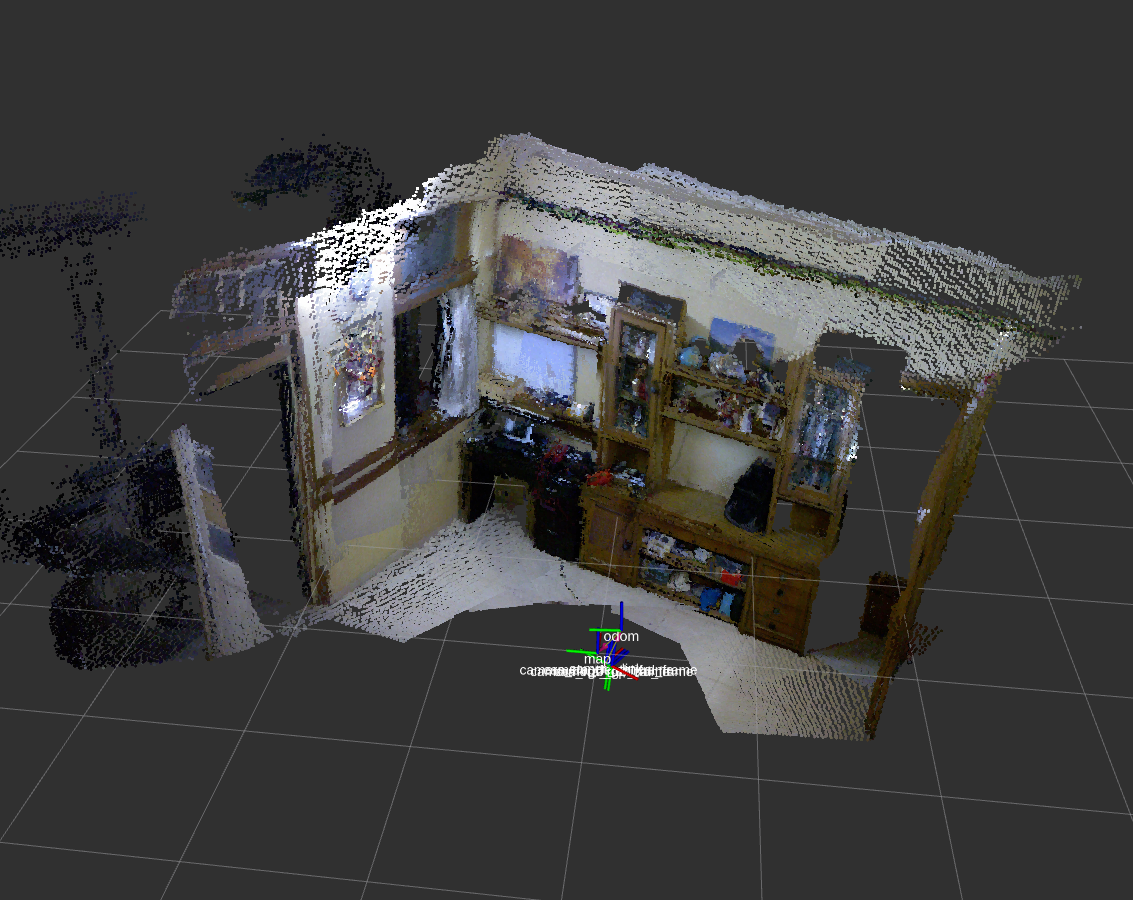
\includegraphics[width=2.5in]{1(1).png}
\caption{Mapping results with laptop}
\label{fig_sim}
\end{figure}
 
\begin{figure}[ht]
	\centering
	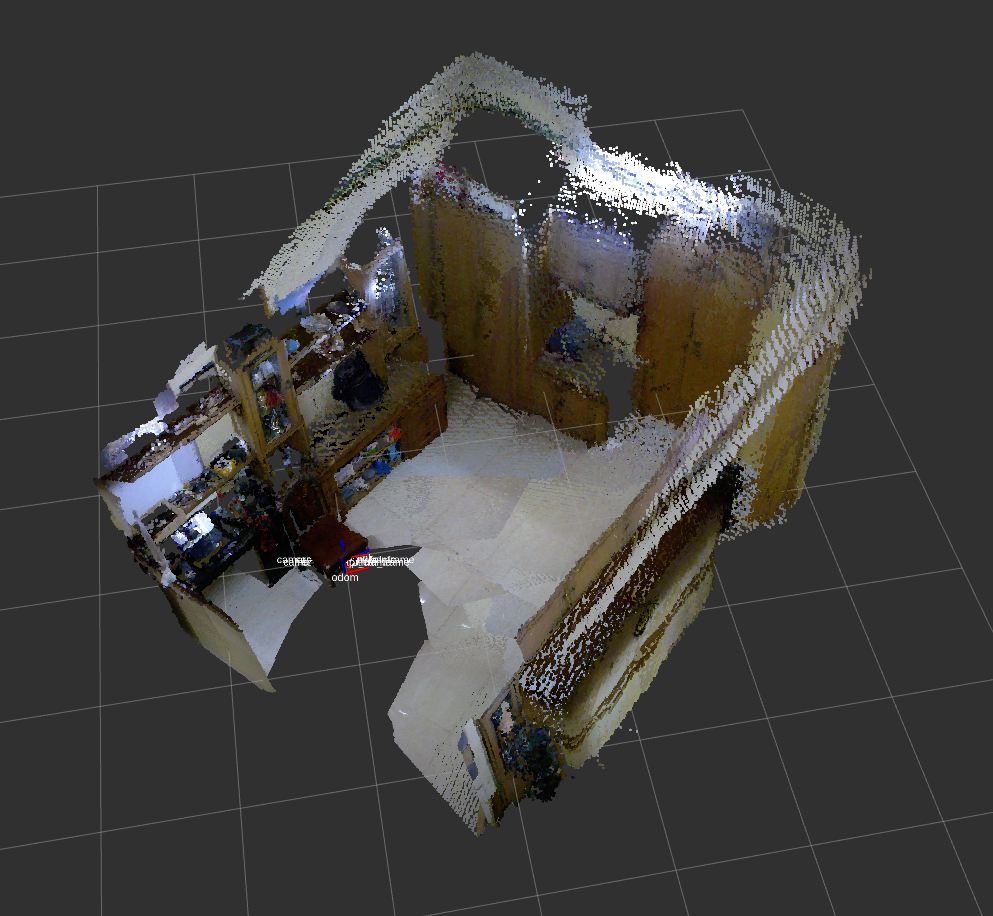
\includegraphics[width=2.5in]{1(2).png}
	\caption{Mapping results with laptop}
	\label{fig_sim}
\end{figure}

\begin{figure}[ht]
	\centering
	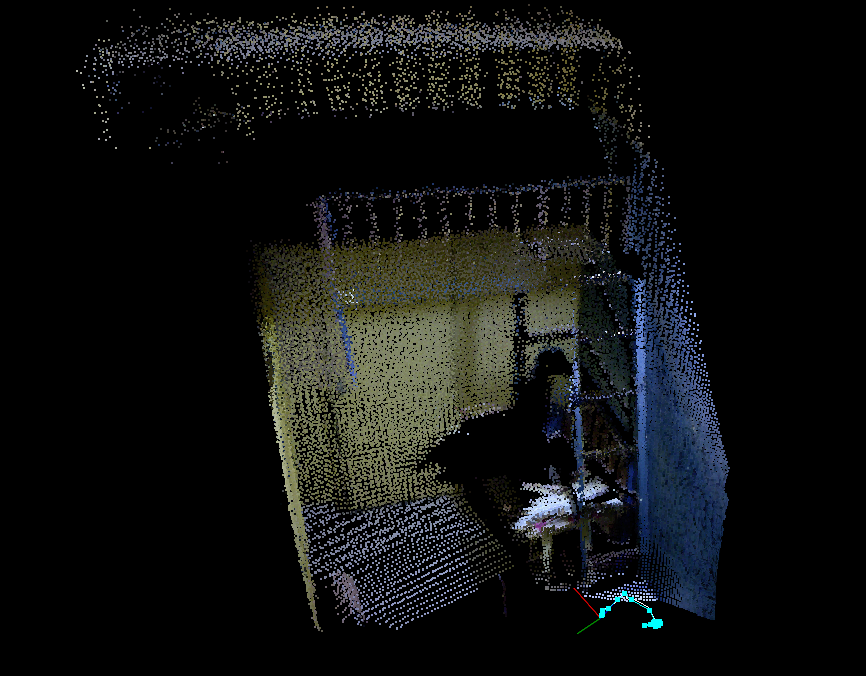
\includegraphics[width=2.5in]{2(1).png}
	\caption{Wireless Mapping with Raspberry Pi}
	\label{fig_sim}
\end{figure}

\begin{figure}[ht]
	\centering
	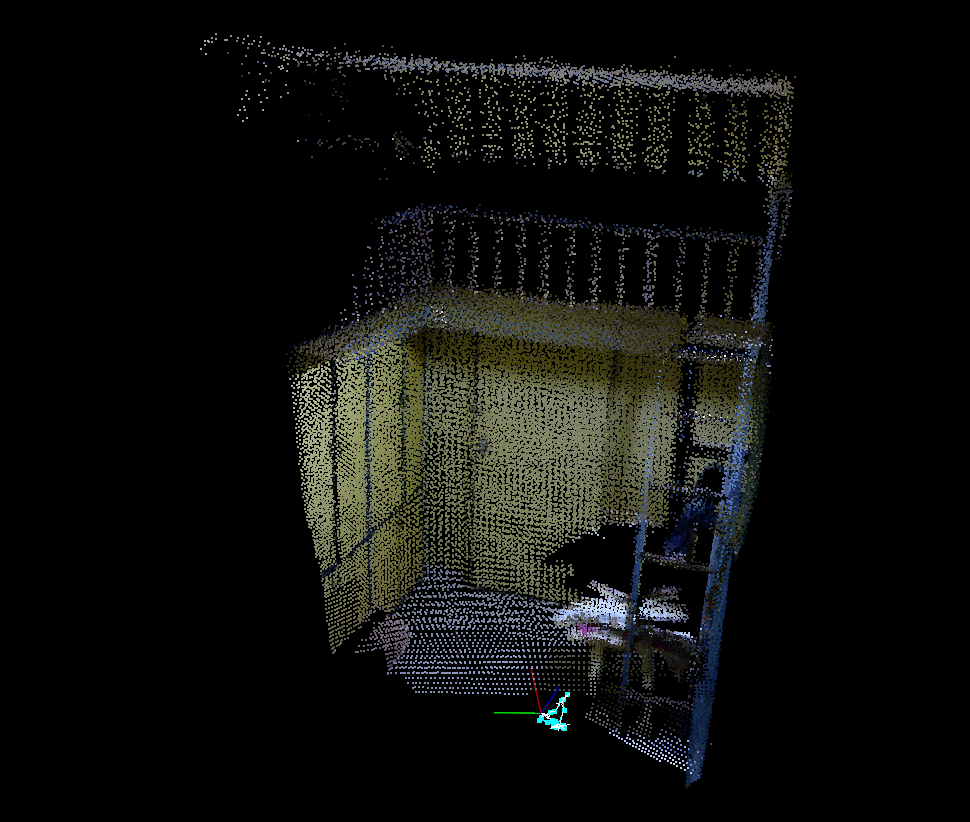
\includegraphics[width=2.5in]{2(2).png}
	\caption{Wireless Mapping with Raspberry Pi}
	\label{fig_sim}
\end{figure}

\section{Conclusion}
The conclusion goes here.





% if have a single appendix:
%\appendix[Proof of the Zonklar Equations]
% or
%\appendix  % for no appendix heading
% do not use \section anymore after \appendix, only \section*
% is possibly needed

% use appendices with more than one appendix
% then use \section to start each appendix
% you must declare a \section before using any
% \subsection or using \label (\appendices by itself
% starts a section numbered zero.)
%


\appendices
\section{Proof of the First Zonklar Equation}
Appendix one text goes here.

% you can choose not to have a title for an appendix
% if you want by leaving the argument blank
\section{}
Appendix two text goes here.


% use section* for acknowledgment
\section*{Acknowledgment}


The authors would like to thank...


% Can use something like this to put references on a page
% by themselves when using endfloat and the captionsoff option.
\ifCLASSOPTIONcaptionsoff
  \newpage
\fi



% trigger a \newpage just before the given reference
% number - used to balance the columns on the last page
% adjust value as needed - may need to be readjusted if
% the document is modified later
%\IEEEtriggeratref{8}
% The "triggered" command can be changed if desired:
%\IEEEtriggercmd{\enlargethispage{-5in}}

% references section

% can use a bibliography generated by BibTeX as a .bbl file
% BibTeX documentation can be easily obtained at:
% http://mirror.ctan.org/biblio/bibtex/contrib/doc/
% The IEEEtran BibTeX style support page is at:
% http://www.michaelshell.org/tex/ieeetran/bibtex/
%\bibliographystyle{IEEEtran}
% argument is your BibTeX string definitions and bibliography database(s)
%\bibliography{IEEEabrv,../bib/paper}
%
% <OR> manually copy in the resultant .bbl file
% set second argument of \begin to the number of references
% (used to reserve space for the reference number labels box)
\begin{thebibliography}{1}

\bibitem{IEEEhowto:kopka}
H.~Kopka and P.~W. Daly, \emph{A Guide to \LaTeX}, 3rd~ed.\hskip 1em plus
  0.5em minus 0.4em\relax Harlow, England: Addison-Wesley, 1999.

\end{thebibliography}

% biography section
% 
% If you have an EPS/PDF photo (graphicx package needed) extra braces are
% needed around the contents of the optional argument to biography to prevent
% the LaTeX parser from getting confused when it sees the complicated
% \includegraphics command within an optional argument. (You could create
% your own custom macro containing the \includegraphics command to make things
% simpler here.)
%\begin{IEEEbiography}[{\includegraphics[width=1in,height=1.25in,clip,keepaspectratio]{mshell}}]{Michael Shell}
% or if you just want to reserve a space for a photo:
\end{document}


